\documentclass[12pt,a4paper]{article}
\usepackage[utf8]{vietnam}
\usepackage{amsmath,amssymb,amsfonts,mathrsfs}
\usepackage[left=1.5cm,right=1.5cm,top=2cm,bottom=2cm,headheight=17pt]{geometry}
\usepackage{enumitem}
\usepackage{array}
\usepackage{graphicx}
\usepackage{tikz}
\usetikzlibrary{arrows.meta,calc,patterns}
\usepackage{fancyhdr}

\pagestyle{fancy}
\fancyhf{}
\lhead{\small\textbf{HƯỚNG TỚI THPTQG 2027}}
\rhead{\small\textit{Người biên soạn: Dương Gia Bảo}}
\rfoot{\small Trang \thepage}
\renewcommand{\headrulewidth}{0.4pt}

\begin{document}

\noindent
\begin{minipage}[t]{0.40\textwidth}
    \centering
    \textbf{HƯỚNG TỚI THPTQG 2027}\\[-2pt]
    \rule{3.2cm}{0.6pt}\\[4pt]
    \textbf{ĐỀ CHÍNH THỨC}
\end{minipage}\hfill
\begin{minipage}[t]{0.58\textwidth}
    \centering
    \textbf{ĐỀ THI KHẢO SÁT CHẤT LƯỢNG}\\
    \textbf{ĐỀ SỐ 9}\\
    \textbf{Môn thi: TOÁN}\\
    \textit{\small Thời gian làm bài: 90 phút, không kể thời gian phát đề}
\end{minipage}

\vspace{0.2cm}
\noindent
\begin{minipage}[b]{0.78\textwidth}
    \textbf{Họ và tên:}\dotfill\textbf{SBD:}\makebox[3.5cm]{\dotfill}
\end{minipage}\hfill
\begin{minipage}[b]{0.20\textwidth}
    \hfill
    \setlength{\fboxrule}{0.8pt}%
    \fbox{\begin{minipage}{2.3cm}
        \centering
        \textbf{\small Mã đề thi}\\
        \textbf{0009}
    \end{minipage}}
\end{minipage}
\vspace{0.2cm}

% ==========================================
% PHẦN I
% ==========================================
\section*{\large PHẦN I. CÂU TRẮC NGHIỆM NHIỀU PHƯƠNG ÁN LỰA CHỌN}
\textit{Thí sinh trả lời từ câu 1 đến câu 12. Mỗi câu hỏi thí sinh chỉ chọn một phương án. Mỗi câu trả lời đúng được 0,25 điểm.}

\begin{enumerate}[label=\textbf{Câu \arabic*:}, leftmargin=*]

\item Cho hàm số $y = \dfrac{x^2 - 4x + 7}{x - 2}$ có đồ thị $(C)$. Tâm đối xứng của đồ thị $(C)$ là điểm
\begin{enumerate}[label=\Alph*.]
    \item $I(2; 0)$.
    \item $I(-2; 0)$.
    \item $I(2; -2)$.
    \item $I(0; -2)$.
\end{enumerate}

\item Có bao nhiêu số nguyên $x \in [-5; 10]$ thỏa mãn bất phương trình $\log_2(x^2 - 3x + 2) \le 1 + \log_2(x + 2)$?
\begin{enumerate}[label=\Alph*.]
    \item $6$.
    \item $5$.
    \item $4$.
    \item $3$.
\end{enumerate}

\item Cho tích phân $\displaystyle \int_0^2 (2x + 1) e^x \mathrm{d}x = a \cdot e^2 + b$ với $a, b \in \mathbb{Z}$. Tổng $a + b$ bằng
\begin{enumerate}[label=\Alph*.]
    \item $5$.
    \item $4$.
    \item $2$.
    \item $3$.
\end{enumerate}

\item Trong không gian $Oxyz$, cho mặt phẳng $(P): 2x - y + 2z - 5 = 0$ và điểm $A(1; 3; -2)$. Khoảng cách từ điểm $A$ đến mặt phẳng $(P)$ bằng
\begin{enumerate}[label=\Alph*.]
    \item $\dfrac{8}{3}$.
    \item $2$.
    \item $\dfrac{4}{3}$.
    \item $\dfrac{10}{3}$.
\end{enumerate}

\item Một hộp chứa 6 quả cầu màu đỏ và 4 quả cầu màu xanh có kích thước và khối lượng như nhau. Lấy ngẫu nhiên lần lượt 2 quả cầu (không hoàn lại). Xác suất để quả cầu lấy ra ở lần thứ hai có màu đỏ, biết rằng quả cầu lấy ra ở lần thứ nhất có màu xanh bằng
\begin{enumerate}[label=\Alph*.]
    \item $\dfrac{2}{3}$.
    \item $\dfrac{3}{5}$.
    \item $\dfrac{1}{2}$.
    \item $\dfrac{4}{9}$.
\end{enumerate}

\item Khảo sát thời gian hoàn thành bài kiểm tra trực tuyến (đơn vị: phút) của 40 học sinh thu được bảng số liệu ghép nhóm sau:
\begin{center}
\begin{tabular}{|c|c|c|c|c|c|}
\hline
\textbf{Thời gian (phút)} & $[15; 20)$ & $[20; 25)$ & $[25; 30)$ & $[30; 35)$ & $[35; 40)$ \\ \hline
\textbf{Số học sinh} & 4 & 12 & 14 & 8 & 2 \\ \hline
\end{tabular}
\end{center}
Trung vị $M_e$ của mẫu số liệu ghép nhóm trên bằng
\begin{enumerate}[label=\Alph*.]
    \item $\dfrac{180}{7}$.
    \item $26$.
    \item $\dfrac{185}{7}$.
    \item $\dfrac{190}{7}$.
\end{enumerate}

\item Cho hình lăng trụ đứng $ABC.A'B'C'$ có đáy $ABC$ là tam giác vuông tại $B$, $AB = a$, $BC = a\sqrt{3}$ và cạnh bên $AA' = 2a$. Tang của góc giữa đường thẳng $A'C$ và mặt phẳng đáy $(ABC)$ bằng
\begin{enumerate}[label=\Alph*.]
    \item $\sqrt{3}$.
    \item $1$.
    \item $\dfrac{\sqrt{3}}{3}$.
    \item $2$.
\end{enumerate}

\item Cho cấp số cộng $(u_n)$ có số hạng đầu $u_1 = 3$ và số hạng thứ năm $u_5 = 15$. Tổng của 20 số hạng đầu tiên $S_{20}$ của cấp số cộng đó bằng
\begin{enumerate}[label=\Alph*.]
    \item $600$.
    \item $660$.
    \item $570$.
    \item $630$.
\end{enumerate}

\item Một chất điểm chuyển động theo phương thẳng đứng với vận tốc $v(t) = 3t^2 + 2t + 1$ (m/s), trong đó $t$ là thời gian tính bằng giây ($t \ge 0$). Quãng đường chất điểm đi được từ thời điểm $t = 0$ đến thời điểm mà gia tốc của nó đạt $14\text{ m/s}^2$ bằng
\begin{enumerate}[label=\Alph*.]
    \item $14\text{ m}$.
    \item $12\text{ m}$.
    \item $16\text{ m}$.
    \item $10\text{ m}$.
\end{enumerate}

\item Trong không gian $Oxyz$, phương trình của mặt cầu $(S)$ có tâm $I(2; -1; 4)$ và đi qua điểm $A(1; 1; 2)$ là
\begin{enumerate}[label=\Alph*.]
    \item $(x + 2)^2 + (y - 1)^2 + (z + 4)^2 = 9$.
    \item $(x - 2)^2 + (y + 1)^2 + (z - 4)^2 = 3$.
    \item $(x - 2)^2 + (y + 1)^2 + (z - 4)^2 = 9$.
    \item $(x + 2)^2 + (y - 1)^2 + (z + 4)^2 = 3$.
\end{enumerate}

\item Một doanh nghiệp sản xuất một loại sản phẩm với hàm tổng chi phí $C(x) = x^3 - 30x^2 + 400x + 500$ (nghìn đồng), trong đó $x \in [5; 25]$ là số lượng sản phẩm sản xuất. Chi phí biên $C'(x)$ đạt giá trị nhỏ nhất khi mức sản lượng $x$ bằng
\begin{enumerate}[label=\Alph*.]
    \item $15$.
    \item $10$.
    \item $20$.
    \item $5$.
\end{enumerate}

\item Cho hình chóp $S.ABC$ có $SA \perp (ABC)$, đáy $ABC$ là tam giác đều cạnh $2a$. Góc giữa đường thẳng $SC$ và mặt phẳng đáy $(ABC)$ bằng $60^\circ$. Thể tích của khối chóp $S.ABC$ bằng
\begin{enumerate}[label=\Alph*.]
    \item $\dfrac{2a^3\sqrt{3}}{3}$.
    \item $a^3\sqrt{3}$.
    \item $\dfrac{a^3}{3}$.
    \item $2a^3$.
\end{enumerate}

\end{enumerate}

% ==========================================
% PHẦN II
% ==========================================
\vspace{0.4cm}
\section*{\large PHẦN II. CÂU TRẮC NGHIỆM ĐÚNG SAI}
\textit{Thí sinh trả lời từ câu 1 đến câu 4. Trong mỗi ý \textbf{a)}, \textbf{b)}, \textbf{c)}, \textbf{d)} ở mỗi câu, thí sinh chọn đúng hoặc sai.}
\begin{itemize}[leftmargin=*]
    \item Điểm tối đa của 01 câu hỏi là 1 điểm.
    \item Thí sinh chỉ lựa chọn chính xác 01 ý trong 01 câu hỏi được 0,1 điểm.
    \item Thí sinh chỉ lựa chọn chính xác 02 ý trong 01 câu hỏi được 0,25 điểm.
    \item Thí sinh chỉ lựa chọn chính xác 03 ý trong 01 câu hỏi được 0,5 điểm.
    \item Thí sinh lựa chọn chính xác cả 04 ý trong 01 câu hỏi được 1 điểm.
\end{itemize}

\begin{enumerate}[label=\textbf{Câu \arabic*:}, leftmargin=*]

\item Cho hàm số $y = f(x) = \dfrac{x^2 - 3x + 6}{x - 1}$ có đồ thị $(C)$.
\begin{enumerate}[label=\textbf{\alph*)}]
    \item Hàm số đạt cực tiểu tại $x = 3$ và đạt cực đại tại $x = -1$.
    \item Đường thẳng đi qua hai điểm cực trị của đồ thị hàm số có phương trình $y = 2x - 3$.
    \item Giao điểm của hai đường tiệm cận của đồ thị $(C)$ là điểm $I(1; 1)$.
    \item Khoảng cách từ gốc tọa độ $O$ đến đường tiệm cận xiên của đồ thị $(C)$ bằng $\sqrt{2}$.
\end{enumerate}

\item Một nhà máy sản xuất chip AI sử dụng 3 dây chuyền tự động $I, II, III$. Dây chuyền $I$ cung cấp $50\%$ tổng sản lượng với tỉ lệ phế phẩm là $2\%$; dây chuyền $II$ cung cấp $30\%$ sản lượng với tỉ lệ phế phẩm là $3\%$; dây chuyền $III$ cung cấp $20\%$ sản lượng với tỉ lệ phế phẩm là $5\%$. Tất cả các sản phẩm được lưu kho chung.
\begin{enumerate}[label=\textbf{\alph*)}]
    \item Xác suất để một chip được chọn ngẫu nhiên từ kho là chip đạt chuẩn (không bị lỗi) bằng $0{,}971$.
    \item Nếu chọn ngẫu nhiên một chip từ kho và phát hiện nó bị lỗi, xác suất chip đó do dây chuyền $I$ sản xuất lớn hơn $35\%$.
    \item Xác suất để một chip được chọn ngẫu nhiên vừa do dây chuyền $II$ hoặc $III$ sản xuất, vừa là chip đạt chuẩn bằng $0{,}481$.
    \item Kiểm tra độc lập 2 chip từ kho, xác suất có đúng một chip bị lỗi bằng $0{,}0563$ (kết quả làm tròn đến hàng phần chục nghìn).
\end{enumerate}

\item \begin{minipage}[t]{0.55\linewidth}
Một giàn đèn sân khấu có trọng lượng $P = 60\text{ N}$ được treo cố định tại điểm $S(0; 0; 2)$ trong không gian $Oxyz$ (đơn vị đo trên các trục là mét). Trần nhà là mặt phẳng $(P)$ có phương trình $z = 4$. Giàn đèn được giữ cân bằng bởi ba sợi dây cáp căng nối từ điểm $S$ đến ba điểm cố định trên trần nhà là $A(2; 0; 4)$, $B(-1; \sqrt{3}; 4)$ và $C(-1; -\sqrt{3}; 4)$. Trọng lực tác dụng lên giàn đèn có vectơ $\vec{P} = (0; 0; -60)$.
\begin{enumerate}[label=\textbf{\alph*)}]
    \item Độ dài của mỗi sợi dây cáp treo bằng $2\sqrt{2}\text{ m}$.
    \item Góc nghiêng giữa mỗi sợi dây cáp treo và trần nhà bằng $45^\circ$.
    \item Cosin của góc giữa hai sợi dây cáp $SA$ và $SB$ bằng $\dfrac{1}{2}$.
    \item Lực căng trên mỗi sợi dây cáp có độ lớn bằng $20\sqrt{2}\text{ N}$.
\end{enumerate}
\end{minipage}\hfill
\begin{minipage}[t]{0.42\linewidth}
\vspace{-0.4\baselineskip}
\centering
\resizebox{\linewidth}{!}{%
\begin{tikzpicture}[>=Stealth, line join=round, line cap=round,
    x={(-0.62cm,-0.36cm)}, y={(1cm,0cm)}, z={(0cm,1cm)}, scale=1.1]
    % Trục tọa độ Oxyz
    \draw[->, thick, gray!70] (0,0,0) -- (3.2,0,0) node[below left, text=black] {$x$};
    \draw[->, thick, gray!70] (0,0,0) -- (0,3.2,0) node[right, text=black] {$y$};
    \draw[->, thick, gray!70] (0,0,0) -- (0,0,5.2) node[above, text=black] {$z$};
    \node[below left] at (0,0,0) {$O$};

    % Mặt phẳng trần nhà z = 4
    \draw[dashed, thin, fill=gray!12, fill opacity=0.4] 
        (-2.2,-2.4,4) -- (2.6,-2.4,4) -- (2.6,2.4,4) -- (-2.2,2.4,4) -- cycle;
    \node[right, font=\footnotesize, text=gray!80!black] at (2.6,2.4,4) {Trần ($z=4$)};

    % Tọa độ các điểm
    \coordinate (A) at (2,0,4);
    \coordinate (B) at (-1,1.732,4);
    \coordinate (C) at (-1,-1.732,4);
    \coordinate (S) at (0,0,2);

    % Ba sợi dây cáp
    \draw[very thick, blue!65!black] (S) -- (A);
    \draw[very thick, blue!65!black] (S) -- (B);
    \draw[very thick, blue!65!black] (S) -- (C);

    % Vectơ trọng lực P
    \draw[->, very thick, red!85!black] (S) -- (0,0,0.5) node[right, font=\small] {$\vec{P}$};

    % Các điểm mốc
    \filldraw (A) circle (1.8pt) node[above right, fill=white, inner sep=1pt] {$A$};
    \filldraw (B) circle (1.8pt) node[above, fill=white, inner sep=1pt] {$B$};
    \filldraw (C) circle (1.8pt) node[below left, fill=white, inner sep=1pt] {$C$};
    \filldraw[fill=orange!85!yellow, draw=black, thick] (S) circle (3pt) node[left, fill=white, inner sep=1pt] {$S$};
\end{tikzpicture}%
}
\end{minipage}

\item Khảo sát thành tích chạy 100 mét (đơn vị: giây) của hai nhóm gồm 40 học sinh lớp 12A và 40 học sinh lớp 12B thu được bảng phân bố tần số ghép nhóm sau:
\begin{center}
\begin{tabular}{|c|c|c|c|c|c|}
\hline
\textbf{Thời gian (giây)} & $[12; 13)$ & $[13; 14)$ & $[14; 15)$ & $[15; 16)$ & $[16; 17)$ \\ \hline
\textbf{Số học sinh lớp 12A} & 5 & 18 & 11 & 4 & 2 \\ \hline
\textbf{Số học sinh lớp 12B} & 3 & 19 & 14 & 3 & 1 \\ \hline
\end{tabular}
\end{center}
\begin{enumerate}[label=\textbf{\alph*)}]
    \item Thời gian chạy trung bình của học sinh lớp 12A bằng $14{,}0$ giây.
    \item Phương sai của mẫu số liệu ghép nhóm của lớp 12A bằng $1{,}2$.
    \item Độ lệch chuẩn của mẫu số liệu ghép nhóm của lớp 12B nhỏ hơn độ lệch chuẩn của lớp 12A.
    \item Học sinh lớp 12B có thành tích chạy 100 mét đồng đều hơn học sinh lớp 12A.
\end{enumerate}

\end{enumerate}

% ==========================================
% PHẦN III
% ==========================================
\vspace{0.4cm}
\section*{\large PHẦN III. CÂU TRẮC NGHIỆM TRẢ LỜI NGẮN}
\textit{Thí sinh trả lời từ câu 1 đến câu 6. Mỗi câu trả lời đúng được 0,5 điểm.}

\begin{enumerate}[label=\textbf{Câu \arabic*:}, leftmargin=*]

\item Một bể nước hình hộp chữ nhật có kích thước đáy là $6\text{ dm} \times 8\text{ dm}$ và chiều cao bằng $10\text{ dm}$. Một chú ốc sên bò trên bề mặt bên ngoài của bể từ đỉnh góc dưới $A$ đến đỉnh góc đối diện trên cùng $C'$. Quãng đường ngắn nhất mà chú ốc sên cần bò bằng bao nhiêu đề-xi-mét? (kết quả làm tròn đến hàng phần mười).

\item \begin{minipage}[t]{0.55\linewidth}
Một cổng chào triển lãm có thiết kế gồm hai đường biên cong dạng parabol đối xứng qua trục tung $Oy$ như hình vẽ bên. Đường cong phía trên có phương trình $y = 9 - x^2$ và đường cong phía dưới có phương trình $y = 6 - \dfrac{2}{3}x^2$ (đơn vị trên các trục là mét, với $-3 \le x \le 3$). Phần vòm ở giữa hai đường cong (phần gạch chéo) được ốp bằng gạch gốm mỹ thuật, phần phía dưới được dành làm lối đi thông thoáng. Diện tích của phần vòm được ốp gạch gốm mỹ thuật bằng bao nhiêu mét vuông?
\end{minipage}\hfill
\begin{minipage}[t]{0.42\linewidth}
\vspace{-0.4\baselineskip}
\centering
\resizebox{\linewidth}{!}{%
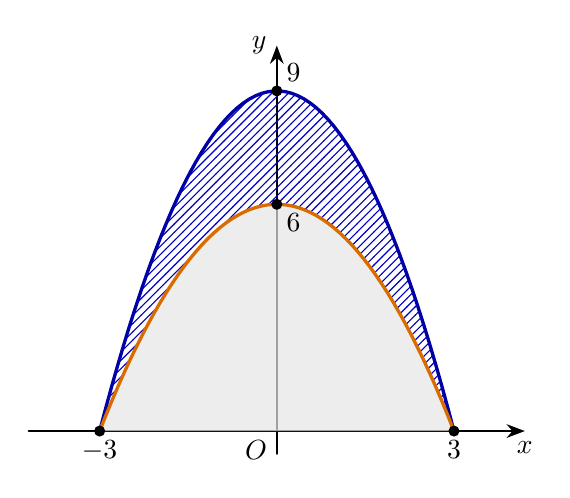
\begin{tikzpicture}[>=Stealth, x=0.75cm, y=0.48cm, line join=round, line cap=round]
    % Trục tọa độ
    \draw[->, thick] (-4.2,0) -- (4.2,0) node[below] {$x$};
    \draw[->, thick] (0,-0.6) -- (0,10.2) node[left] {$y$};
    \node[below left] at (0,0) {$O$};

    % Miền gạch chéo giữa 2 parabol (kín chuẩn từ -3 đến 3)
    \fill[pattern=north east lines, pattern color=blue!75!black, domain=-3:3, samples=50] 
        plot (\x, {9 - (\x)^2}) -- 
        plot (-\x, {6 - (2/3)*(-\x)^2}) -- cycle;

    % Miền dưới tô xám nhạt (lối đi thông thoáng)
    \fill[gray!20, opacity=0.7, domain=-3:3, samples=50] 
        plot (\x, {6 - (2/3)*(\x)^2}) -- (3,0) -- (-3,0) -- cycle;

    % Hai đường parabol kết thúc chuẩn xác tại mặt đất y = 0
    \draw[very thick, blue!65!black, domain=-3:3, samples=60] plot (\x, {9 - (\x)^2});
    \draw[very thick, orange!85!black, domain=-3:3, samples=60] plot (\x, {6 - (2/3)*(\x)^2});

    % Tọa độ các mốc
    \node[below] at (-3,0) {$-3$};
    \node[below] at (3,0) {$3$};
    \fill (0,9) circle (2pt) node[above right] {$9$};
    \fill (0,6) circle (2pt) node[below right] {$6$};
    \fill (-3,0) circle (2pt);
    \fill (3,0) circle (2pt);
\end{tikzpicture}%
}
\end{minipage}

\item Một xưởng thủ công mỹ nghệ sản xuất một loại bàn ghế gỗ cao cấp. Khi xưởng bán sản phẩm với giá $p$ (nghìn đồng/sản phẩm) thì hàm cầu của thị trường là $p(x) = 200 - x$, trong đó $x$ là số lượng sản phẩm tiêu thụ được ($0 \le x \le 150$). Chi phí để sản xuất $x$ sản phẩm là $C(x) = x^2 + 32x + 800$ (nghìn đồng). Nhà nước áp thuế môi trường $8$ nghìn đồng trên mỗi sản phẩm bán ra. Lợi nhuận lớn nhất mà xưởng có thể đạt được sau khi nộp thuế bằng bao nhiêu nghìn đồng?

\item Trong không gian $Oxyz$, cho mặt cầu $(S): (x - 1)^2 + (y - 2)^2 + (z - 3)^2 = 9$ và điểm cố định $A(3; 5; 9)$. Điểm $M$ thay đổi trên bề mặt của mặt cầu $(S)$. Khoảng cách ngắn nhất giữa điểm $A$ và điểm $M$ bằng bao nhiêu?

\item Một hệ thống truyền tin số phát các gói dữ liệu dưới dạng bit $0$ và bit $1$. Thống kê cho thấy xác suất phát bit $0$ là $0{,}6$ và xác suất phát bit $1$ là $0{,}4$. Do ảnh hưởng của nhiễu trên đường truyền, một bit $0$ khi phát đi có xác suất $0{,}05$ bị nhận nhầm thành bit $1$; trong khi một bit $1$ khi phát đi có xác suất $0{,}10$ bị nhận nhầm thành bit $0$. Biết rằng đầu thu vừa nhận được một bit $1$, xác suất để bit thực sự được gửi đi từ đầu phát là bit $1$ bằng bao nhiêu? (kết quả làm tròn đến hàng phần trăm).

\item Một bồn chứa nhiên liệu dạng vật thể được đặt nằm ngang giữa hai mặt phẳng có phương trình $x = 0$ và $x = 6$. Cắt bồn chứa bởi một mặt phẳng vuông góc với trục $Ox$ tại điểm có hoành độ $x$ ($0 \le x \le 6$), thiết diện thu được luôn là một hình vuông có độ dài cạnh bằng $\sqrt{36 - x^2}$ (mét). Thể tích của bồn chứa nhiên liệu đó bằng bao nhiêu mét khối?

\end{enumerate}

% ==========================================
% BẢNG ĐÁP ÁN TỔNG HỢP
% ==========================================
\newpage
\begin{center}
    \textbf{\Large BẢNG ĐÁP ÁN TỔNG HỢP ĐỀ SỐ 9}
\end{center}

\vspace{0.4cm}
\noindent\textbf{\large PHẦN I: CÂU TRẮC NGHIỆM NHIỀU PHƯƠNG ÁN LỰA CHỌN}
\begin{center}
\renewcommand{\arraystretch}{1.3}
\begin{tabular}{|c|c|c|c|c|c|c|c|c|c|c|c|}
\hline
\textbf{1} & \textbf{2} & \textbf{3} & \textbf{4} & \textbf{5} & \textbf{6} & \textbf{7} & \textbf{8} & \textbf{9} & \textbf{10} & \textbf{11} & \textbf{12} \\ \hline
\textbf{A} & \textbf{C} & \textbf{B} & \textbf{D} & \textbf{A} & \textbf{C} & \textbf{B} & \textbf{D} & \textbf{A} & \textbf{C} & \textbf{B} & \textbf{D} \\ \hline
\end{tabular}
\end{center}
\textit{Thống kê phương án Phần I: $3\text{A} - 3\text{B} - 3\text{C} - 3\text{D}$ (phân bố đều tuyệt đối).}

\vspace{0.5cm}
\noindent\textbf{\large PHẦN II: CÂU TRẮC NGHIỆM ĐÚNG SAI}
\begin{center}
\renewcommand{\arraystretch}{1.3}
\begin{tabular}{|c|c|c|c|c|}
\hline
\textbf{Ý / Câu} & \textbf{Câu 1} & \textbf{Câu 2} & \textbf{Câu 3} & \textbf{Câu 4} \\ \hline
\textbf{a)} & \textbf{Đ} & \textbf{Đ} & \textbf{Đ} & \textbf{Đ} \\ \hline
\textbf{b)} & \textbf{Đ} & \textbf{S} & \textbf{Đ} & \textbf{S} \\ \hline
\textbf{c)} & \textbf{S} & \textbf{Đ} & \textbf{S} & \textbf{Đ} \\ \hline
\textbf{d)} & \textbf{Đ} & \textbf{Đ} & \textbf{Đ} & \textbf{Đ} \\ \hline
\end{tabular}
\end{center}

\vspace{0.5cm}
\noindent\textbf{\large PHẦN III: CÂU TRẮC NGHIỆM TRẢ LỜI NGẮN}
\begin{center}
\renewcommand{\arraystretch}{1.4}
\begin{tabular}{|c|c|c|c|c|c|}
\hline
\textbf{Câu 1} & \textbf{Câu 2} & \textbf{Câu 3} & \textbf{Câu 4} & \textbf{Câu 5} & \textbf{Câu 6} \\ \hline
\textbf{17,2} & \textbf{12} & \textbf{2400} & \textbf{4} & \textbf{0,92} & \textbf{144} \\ \hline
\end{tabular}
\end{center}

% ==========================================
% HƯỚNG DẪN GIẢI CHI TIẾT
% ==========================================
\newpage
\begin{center}
    \textbf{\Large HƯỚNG DẪN GIẢI CHI TIẾT}
\end{center}
\vspace{0.3cm}

\subsection*{\large PHẦN I. CÂU TRẮC NGHIỆM NHIỀU PHƯƠNG ÁN LỰA CHỌN}

\noindent\textbf{Câu 1.} Chọn \textbf{A}.\\
Biến đổi hàm số: $y = \dfrac{x^2 - 4x + 7}{x - 2} = x - 2 + \dfrac{3}{x - 2}$.
\begin{itemize}[leftmargin=*]
    \item Tiệm cận đứng: $x = 2$.
    \item Tiệm cận xiên: $y = x - 2$.
    \item Giao điểm của hai đường tiệm cận là nghiệm của hệ $\begin{cases} x = 2 \\ y = x - 2 \end{cases} \iff \begin{cases} x = 2 \\ y = 0 \end{cases} \implies I(2; 0)$.
\end{itemize}
Điểm $I(2; 0)$ chính là tâm đối xứng của đồ thị $(C)$.\hfill$\blacksquare$

\vspace{0.2cm}\noindent\textbf{Câu 2.} Chọn \textbf{C}.\\
Điều kiện xác định:
$\begin{cases} x^2 - 3x + 2 > 0 \\ x + 2 > 0 \end{cases} \iff \begin{cases} x \in (-\infty; 1) \cup (2; +\infty) \\ x > -2 \end{cases} \iff x \in (-2; 1) \cup (2; +\infty)$.\\
Bất phương trình đã cho tương đương với:
$$\log_2(x^2 - 3x + 2) \le \log_2[2(x + 2)] \iff x^2 - 3x + 2 \le 2x + 4 \iff x^2 - 5x - 2 \le 0$$
$$\iff \dfrac{5 - \sqrt{33}}{2} \le x \le \dfrac{5 + \sqrt{33}}{2} \quad (\text{vì } \sqrt{33} \approx 5{,}744 \text{ nên } -0{,}372 \le x \le 5{,}372).$$
Kết hợp với điều kiện xác định $x \in (-2; 1) \cup (2; +\infty)$ và $x \in [-5; 10]$, ta được:
$$x \in \left[\dfrac{5 - \sqrt{33}}{2}; 1\right) \cup \left(2; \dfrac{5 + \sqrt{33}}{2}\right].$$
Vì $x \in \mathbb{Z}$ nên:
\begin{itemize}[leftmargin=*]
    \item Trên $\left[\dfrac{5 - \sqrt{33}}{2}; 1\right)$, ta có $x \in \{0\}$.
    \item Trên $\left(2; \dfrac{5 + \sqrt{33}}{2}\right]$, ta có $x \in \{3; 4; 5\}$.
\end{itemize}
Vậy có đúng $4$ số nguyên thỏa mãn yêu cầu bài toán.\hfill$\blacksquare$

\vspace{0.2cm}\noindent\textbf{Câu 3.} Chọn \textbf{B}.\\
Sử dụng phương pháp tích phân từng phần:
Đặt $\begin{cases} u = 2x + 1 \\ \mathrm{d}v = e^x \mathrm{d}x \end{cases} \implies \begin{cases} \mathrm{d}u = 2 \mathrm{d}x \\ v = e^x \end{cases}$.\\
Khi đó:
$$I = \left[(2x + 1)e^x\right]_0^2 - \int_0^2 2e^x \mathrm{d}x = \left[(2x + 1)e^x - 2e^x\right]_0^2 = \left[(2x - 1)e^x\right]_0^2 = 3e^2 - (-1) = 3e^2 + 1.$$
Do đó $a = 3$, $b = 1 \implies a + b = 3 + 1 = 4$.\hfill$\blacksquare$

\vspace{0.2cm}\noindent\textbf{Câu 4.} Chọn \textbf{D}.\\
Áp dụng công thức khoảng cách từ điểm $A(1; 3; -2)$ đến mặt phẳng $(P): 2x - y + 2z - 5 = 0$:
$$d(A, (P)) = \dfrac{|2(1) - 3 + 2(-2) - 5|}{\sqrt{2^2 + (-1)^2 + 2^2}} = \dfrac{|2 - 3 - 4 - 5|}{\sqrt{9}} = \dfrac{|-10|}{3} = \dfrac{10}{3}.\hfill\blacksquare$$

\vspace{0.2cm}\noindent\textbf{Câu 5.} Chọn \textbf{A}.\\
Gọi $A$ là biến cố: ``Quả cầu lấy lần 1 có màu xanh''.\\
Gọi $B$ là biến cố: ``Quả cầu lấy lần 2 có màu đỏ''.\\
Khi quả cầu thứ nhất có màu xanh được lấy ra, trong hộp còn lại $6$ quả màu đỏ và $3$ quả màu xanh (tổng cộng còn 9 quả).\\
Do đó xác suất để quả thứ hai có màu đỏ khi biết quả thứ nhất màu xanh là:
$$P(B|A) = \dfrac{6}{6 + 3} = \dfrac{6}{9} = \dfrac{2}{3}.\hfill\blacksquare$$

\vspace{0.2cm}\noindent\textbf{Câu 6.} Chọn \textbf{C}.\\
Cỡ mẫu $n = 4 + 12 + 14 + 8 + 2 = 40$. Ta có $\dfrac{n}{2} = 20$.\\
Bảng tần số tích lũy:
\begin{center}
\begin{tabular}{|c|c|c|c|c|c|}
\hline
Nhóm & $[15; 20)$ & $[20; 25)$ & $[25; 30)$ & $[30; 35)$ & $[35; 40)$ \\ \hline
Tần số tích lũy $cf_i$ & 4 & 16 & 30 & 38 & 40 \\ \hline
\end{tabular}
\end{center}
Do $cf_2 = 16 < 20 \le 30 = cf_3$ nên nhóm chứa trung vị là nhóm thứ 3: $[25; 30)$.\\
Ta có: $L = 25$, $cf_{k-1} = 16$, $f_k = 14$, $h = 5$.\\
Áp dụng công thức tính trung vị của mẫu số liệu ghép nhóm:
$$M_e = 25 + \dfrac{20 - 16}{14} \cdot 5 = 25 + \dfrac{20}{14} = 25 + \dfrac{10}{7} = \dfrac{185}{7}.\hfill\blacksquare$$

\vspace{0.2cm}\noindent\textbf{Câu 7.} Chọn \textbf{B}.\\
Vì $A'A \perp (ABC)$ nên hình chiếu vuông góc của $A'C$ lên mặt phẳng $(ABC)$ là đoạn thẳng $AC$.\\
Do đó, góc giữa đường thẳng $A'C$ và mặt phẳng đáy $(ABC)$ là góc $\widehat{A'CA}$.\\
Tam giác $ABC$ vuông tại $B$ nên $AC = \sqrt{AB^2 + BC^2} = \sqrt{a^2 + 3a^2} = 2a$.\\
Tam giác $A'AC$ vuông tại $A$ có $A'A = 2a$ và $AC = 2a \implies \tan \widehat{A'CA} = \dfrac{A'A}{AC} = \dfrac{2a}{2a} = 1$.\hfill$\blacksquare$

\vspace{0.2cm}\noindent\textbf{Câu 8.} Chọn \textbf{D}.\\
Ta có $u_5 = u_1 + 4d \iff 15 = 3 + 4d \iff 4d = 12 \iff d = 3$.\\
Tổng 20 số hạng đầu tiên của cấp số cộng:
$$S_{20} = \dfrac{20}{2} \cdot \left[2u_1 + (20 - 1)d\right] = 10 \cdot [2(3) + 19(3)] = 10 \cdot [6 + 57] = 630.\hfill\blacksquare$$

\vspace{0.2cm}\noindent\textbf{Câu 9.} Chọn \textbf{A}.\\
Gia tốc tức thời của chất điểm tại thời điểm $t$ là $a(t) = v'(t) = 6t + 2$.\\
Gia tốc đạt $14\text{ m/s}^2 \iff 6t + 2 = 14 \iff 6t = 12 \iff t = 2\text{ (s)}$.\\
Vì $v(t) = 3t^2 + 2t + 1 > 0$ với mọi $t \ge 0$ nên chất điểm luôn chuyển động theo một chiều.\\
Quãng đường đi được từ $t = 0$ đến $t = 2$ là:
$$s = \int_0^2 (3t^2 + 2t + 1) \mathrm{d}t = \left[t^3 + t^2 + t\right]_0^2 = (8 + 4 + 2) - 0 = 14\text{ (m)}.\hfill\blacksquare$$

\vspace{0.2cm}\noindent\textbf{Câu 10.} Chọn \textbf{C}.\\
Bán kính mặt cầu $(S)$ bằng độ dài đoạn thẳng $IA$:
$$R^2 = IA^2 = (1 - 2)^2 + (1 - (-1))^2 + (2 - 4)^2 = (-1)^2 + 2^2 + (-2)^2 = 1 + 4 + 4 = 9.$$
Phương trình mặt cầu $(S)$ là: $(x - 2)^2 + (y + 1)^2 + (z - 4)^2 = 9$.\hfill$\blacksquare$

\vspace{0.2cm}\noindent\textbf{Câu 11.} Chọn \textbf{B}.\\
Chi phí biên là đạo hàm của hàm tổng chi phí:
$$C'(x) = 3x^2 - 60x + 400.$$
Đây là một hàm số bậc hai có hệ số $a = 3 > 0$ nên đạt giá trị nhỏ nhất tại đỉnh của parabol:
$$x = -\dfrac{b}{2a} = -\dfrac{-60}{2 \cdot 3} = 10 \in [5; 25].$$
Vậy chi phí biên đạt giá trị nhỏ nhất khi mức sản lượng $x = 10$.\hfill$\blacksquare$

\vspace{0.2cm}\noindent\textbf{Câu 12.} Chọn \textbf{D}.\\
Diện tích đáy là tam giác đều cạnh $2a$: $S_{ABC} = \dfrac{(2a)^2\sqrt{3}}{4} = a^2\sqrt{3}$.\\
Vì $SA \perp (ABC)$ nên hình chiếu vuông góc của $SC$ lên đáy là $AC$, do đó $\widehat{SCA} = 60^\circ$.\\
Xét tam giác $SAC$ vuông tại $A$: $SA = AC \cdot \tan 60^\circ = 2a \cdot \sqrt{3} = 2a\sqrt{3}$.\\
Thể tích khối chóp $S.ABC$:
$$V = \dfrac{1}{3} S_{ABC} \cdot SA = \dfrac{1}{3} \cdot (a^2\sqrt{3}) \cdot (2a\sqrt{3}) = 2a^3.\hfill\blacksquare$$

% ------------------------------------------
\subsection*{\large PHẦN II. CÂU TRẮC NGHIỆM ĐÚNG SAI}

\noindent\textbf{Câu 1.}
Tập xác định: $D = \mathbb{R} \setminus \{1\}$. Ta có $f(x) = \dfrac{x^2 - 3x + 6}{x - 1} = x - 2 + \dfrac{4}{x - 1}$.\\
Đạo hàm: $f'(x) = 1 - \dfrac{4}{(x - 1)^2} = \dfrac{(x - 1)^2 - 4}{(x - 1)^2} = \dfrac{x^2 - 2x - 3}{(x - 1)^2}$.\\
Cho $f'(x) = 0 \iff x^2 - 2x - 3 = 0 \iff \left[\begin{array}{l} x = -1 \implies y = -5 \\ x = 3 \implies y = 3 \end{array}\right.$.
\begin{itemize}[leftmargin=*]
    \item \textbf{Ý a) ĐÚNG:} Lập bảng biến thiên thấy hàm số đổi dấu qua $x = -1$ từ dương sang âm nên đạt cực đại tại $x = -1$, đổi dấu qua $x = 3$ từ âm sang dương nên đạt cực tiểu tại $x = 3$.
    \item \textbf{Ý b) ĐÚNG:} Hai điểm cực trị là $A(-1; -5)$ và $B(3; 3)$. Hệ số góc của đường thẳng $AB$ là $k = \dfrac{3 - (-5)}{3 - (-1)} = \dfrac{8}{4} = 2$. Phương trình đường thẳng đi qua hai điểm cực trị là $y - 3 = 2(x - 3) \iff y = 2x - 3$.
    \item \textbf{Ý c) SAI:} Tiệm cận đứng là $x = 1$, tiệm cận xiên là $y = x - 2$. Giao điểm của hai đường tiệm cận là nghiệm của hệ $\begin{cases} x = 1 \\ y = x - 2 \end{cases} \implies I(1; -1)$, không phải $(1; 1)$.
    \item \textbf{Ý d) ĐÚNG:} Đường tiệm cận xiên có dạng tổng quát là $\Delta: x - y - 2 = 0$. Khoảng cách từ $O(0; 0)$ đến $\Delta$ là:
    $$d(O, \Delta) = \dfrac{|0 - 0 - 2|}{\sqrt{1^2 + (-1)^2}} = \dfrac{2}{\sqrt{2}} = \sqrt{2}.\hfill\blacksquare$$
\end{itemize}

\vspace{0.2cm}\noindent\textbf{Câu 2.}
Gọi $A_1, A_2, A_3$ lần lượt là biến cố chip được sản xuất bởi dây chuyền $I, II, III$. Ta có:
$$P(A_1) = 0{,}5; \quad P(A_2) = 0{,}3; \quad P(A_3) = 0{,}2.$$
Gọi $F$ là biến cố ``Chip bị lỗi (phế phẩm)''. Theo đề bài:
$$P(F|A_1) = 0{,}02; \quad P(F|A_2) = 0{,}03; \quad P(F|A_3) = 0{,}05.$$
\begin{itemize}[leftmargin=*]
    \item \textbf{Ý a) ĐÚNG:} Theo công thức xác suất toàn phần:
    $$P(F) = 0{,}5 \cdot 0{,}02 + 0{,}3 \cdot 0{,}03 + 0{,}2 \cdot 0{,}05 = 0{,}010 + 0{,}009 + 0{,}010 = 0{,}029.$$
    Xác suất chọn được chip đạt chuẩn (không bị lỗi) là: $P(\bar{F}) = 1 - 0{,}029 = 0{,}971$.
    \item \textbf{Ý b) SAI:} Theo công thức Bayes, xác suất chip lỗi do dây chuyền $I$ sản xuất là:
    $$P(A_1|F) = \dfrac{P(A_1 \cap F)}{P(F)} = \dfrac{0{,}5 \cdot 0{,}02}{0{,}029} = \dfrac{0{,}010}{0{,}029} = \dfrac{10}{29} \approx 0{,}3448 = 34{,}48\% < 35\%.$$
    \item \textbf{Ý c) ĐÚNG:} Biến cố chip do dây chuyền $II$ hoặc $III$ sản xuất và đạt chuẩn là:
    $$P((A_2 \cup A_3) \cap \bar{F}) = P(A_2) \cdot P(\bar{F}|A_2) + P(A_3) \cdot P(\bar{F}|A_3)$$
    $$= 0{,}3 \cdot (1 - 0{,}03) + 0{,}2 \cdot (1 - 0{,}05) = 0{,}3 \cdot 0{,}97 + 0{,}2 \cdot 0{,}95 = 0{,}291 + 0{,}190 = 0{,}481.$$
    \item \textbf{Ý d) ĐÚNG:} Kiểm tra độc lập 2 chip, xác suất có đúng một chip bị lỗi tuân theo quy tắc nhân biến cố độc lập:
    $$P = 2 \cdot P(F) \cdot P(\bar{F}) = 2 \cdot 0{,}029 \cdot 0{,}971 = 0{,}056318 \approx 0{,}0563.\hfill\blacksquare$$
\end{itemize}

\vspace{0.2cm}\noindent\textbf{Câu 3.}
Ta có tọa độ các điểm: $S(0; 0; 2)$, $A(2; 0; 4)$, $B(-1; \sqrt{3}; 4)$, $C(-1; -\sqrt{3}; 4)$.\\
Các vectơ chỉ phương của 3 sợi dây cáp:
$$\vec{SA} = (2; 0; 2); \quad \vec{SB} = (-1; \sqrt{3}; 2); \quad \vec{SC} = (-1; -\sqrt{3}; 2).$$
\begin{itemize}[leftmargin=*]
    \item \textbf{Ý a) ĐÚNG:} Ta có độ dài mỗi sợi dây cáp:
    $$|\vec{SA}| = \sqrt{2^2 + 0^2 + 2^2} = \sqrt{8} = 2\sqrt{2}\text{ (m)}.$$
    $$|\vec{SB}| = \sqrt{(-1)^2 + (\sqrt{3})^2 + 2^2} = \sqrt{1 + 3 + 4} = 2\sqrt{2}\text{ (m)}.$$
    $$|\vec{SC}| = \sqrt{(-1)^2 + (-\sqrt{3})^2 + 2^2} = \sqrt{1 + 3 + 4} = 2\sqrt{2}\text{ (m)}.$$
    \item \textbf{Ý b) ĐÚNG:} Mặt phẳng trần nhà $z = 4$ có vectơ pháp tuyến $\vec{n} = (0; 0; 1)$.\\
    Góc nghiêng $\alpha$ giữa dây $SA$ và trần nhà thỏa mãn:
    $$\sin \alpha = \dfrac{|\vec{SA} \cdot \vec{n}|}{|\vec{SA}| \cdot |\vec{n}|} = \dfrac{|2(0) + 0(0) + 2(1)|}{2\sqrt{2} \cdot 1} = \dfrac{2}{2\sqrt{2}} = \dfrac{1}{\sqrt{2}} \implies \alpha = 45^\circ.$$
    \item \textbf{Ý c) SAI:} Cosin góc giữa hai sợi cáp $SA$ và $SB$:
    $$\cos(\vec{SA}, \vec{SB}) = \dfrac{2(-1) + 0(\sqrt{3}) + 2(2)}{2\sqrt{2} \cdot 2\sqrt{2}} = \dfrac{-2 + 4}{8} = \dfrac{2}{8} = \dfrac{1}{4} \ne \dfrac{1}{2}.$$
    \item \textbf{Ý d) ĐÚNG:} Gọi lực căng trên mỗi sợi cáp là $\vec{T}_A, \vec{T}_B, \vec{T}_C$. Do tính đối xứng hoàn toàn quanh trục $Oz$, ta có độ lớn lực căng trên ba sợi dây bằng nhau: $|\vec{T}_A| = |\vec{T}_B| = |\vec{T}_C| = T$.\\
    Vectơ lực căng theo hướng dây:
    \begin{align*}
        \vec{T}_A &= T \left(\dfrac{1}{\sqrt{2}}; 0; \dfrac{1}{\sqrt{2}}\right), \\
        \vec{T}_B &= T \left(-\dfrac{1}{2\sqrt{2}}; \dfrac{\sqrt{3}}{2\sqrt{2}}; \dfrac{1}{\sqrt{2}}\right), \quad
        \vec{T}_C = T \left(-\dfrac{1}{2\sqrt{2}}; -\dfrac{\sqrt{3}}{2\sqrt{2}}; \dfrac{1}{\sqrt{2}}\right).
    \end{align*}
    Hệ cân bằng lực: $\vec{T}_A + \vec{T}_B + \vec{T}_C + \vec{P} = \vec{0} \iff \vec{T}_A + \vec{T}_B + \vec{T}_C = (0; 0; 60)$.\\
    Chiếu lên trục $Oz$:
    $$T \left(\dfrac{1}{\sqrt{2}} + \dfrac{1}{\sqrt{2}} + \dfrac{1}{\sqrt{2}}\right) = 60 \iff 3T \cdot \dfrac{1}{\sqrt{2}} = 60 \iff T = \dfrac{60\sqrt{2}}{3} = 20\sqrt{2}\text{ (N)}.\hfill\blacksquare$$
\end{itemize}

\vspace{0.2cm}\noindent\textbf{Câu 4.}
Giá trị đại diện của các nhóm lần lượt là: $x_1 = 12{,}5$; $x_2 = 13{,}5$; $x_3 = 14{,}5$; $x_4 = 15{,}5$; $x_5 = 16{,}5$.
\begin{itemize}[leftmargin=*]
    \item \textbf{Ý a) ĐÚNG:} Thời gian chạy trung bình của học sinh lớp 12A:
    $$\bar{x}_A = \dfrac{5(12{,}5) + 18(13{,}5) + 11(14{,}5) + 4(15{,}5) + 2(16{,}5)}{40} = \dfrac{560}{40} = 14{,}0\text{ (s)}.$$
    \item \textbf{Ý b) SAI:} Phương sai của mẫu số liệu lớp 12A là:
    \begin{align*}
        s_A^2 &= \dfrac{5(12{,}5 - 14)^2 + 18(13{,}5 - 14)^2 + 11(14{,}5 - 14)^2 + 4(15{,}5 - 14)^2 + 2(16{,}5 - 14)^2}{40} \\
        &= \dfrac{11{,}25 + 4{,}5 + 2{,}75 + 9 + 12{,}5}{40} = \dfrac{40}{40} = 1{,}0 \ne 1{,}2.
    \end{align*}
    \item \textbf{Ý c) ĐÚNG:} Với lớp 12B, ta có thời gian trung bình:
    $$\bar{x}_B = \dfrac{3(12{,}5) + 19(13{,}5) + 14(14{,}5) + 3(15{,}5) + 1(16{,}5)}{40} = \dfrac{560}{40} = 14{,}0\text{ (s)}.$$
    Phương sai của mẫu số liệu lớp 12B:
    \begin{align*}
        s_B^2 &= \dfrac{3(12{,}5 - 14)^2 + 19(13{,}5 - 14)^2 + 14(14{,}5 - 14)^2 + 3(15{,}5 - 14)^2 + 1(16{,}5 - 14)^2}{40} \\
        &= \dfrac{6{,}75 + 4{,}75 + 3{,}5 + 6{,}75 + 6{,}25}{40} = \dfrac{28}{40} = 0{,}7.
    \end{align*}
    Độ lệch chuẩn của hai lớp: $s_A = \sqrt{1{,}0} = 1{,}0\text{ (s)}$ và $s_B = \sqrt{0{,}7} \approx 0{,}84\text{ (s)}$. Rõ ràng $s_B < s_A$.
    \item \textbf{Ý d) ĐÚNG:} Cả hai lớp đều có thành tích trung bình bằng nhau ($14{,}0$ giây), nhưng lớp 12B có phương sai và độ lệch chuẩn nhỏ hơn lớp 12A ($0{,}7 < 1{,}0$), chứng tỏ thành tích chạy của học sinh lớp 12B có độ phân tán thấp hơn, tức là đồng đều hơn học sinh lớp 12A.\hfill$\blacksquare$
\end{itemize}

% ------------------------------------------
\subsection*{\large PHẦN III. CÂU TRẮC NGHIỆM TRẢ LỜI NGẮN}

\noindent\textbf{Câu 1.} Đáp số: \textbf{17,2}.\\
Hình hộp chữ nhật có kích thước $a = 6\text{ dm}$, $b = 8\text{ dm}$, $h = 10\text{ dm}$.\\
Để bò từ đỉnh $A$ đến đỉnh đối diện $C'$ trên bề mặt ngoài, khi trải phẳng bề mặt hình hộp lên một mặt phẳng, đoạn thẳng nối $A$ và $C'$ là quãng đường ngắn nhất.\\
Có 3 trường hợp mở trải phẳng tương ứng:
\begin{enumerate}[leftmargin=*]
    \item Trải qua một mặt bên và nắp:\\
    $d_1 = \sqrt{(a + b)^2 + h^2} = \sqrt{(6 + 8)^2 + 10^2} = \sqrt{196 + 100} = \sqrt{296} \approx 17{,}205\text{ dm}$.
    \item Trải qua mặt bên kích thước $a \times h$ và mặt đáy:\\
    $d_2 = \sqrt{(a + h)^2 + b^2} = \sqrt{(6 + 10)^2 + 8^2} = \sqrt{256 + 64} = \sqrt{320} \approx 17{,}889\text{ dm}$.
    \item Trải qua mặt bên kích thước $b \times h$ và mặt đáy:\\
    $d_3 = \sqrt{(b + h)^2 + a^2} = \sqrt{(8 + 10)^2 + 6^2} = \sqrt{324 + 36} = \sqrt{360} \approx 18{,}974\text{ dm}$.
\end{enumerate}
Quãng đường ngắn nhất là $\sqrt{296} = 2\sqrt{74} \approx 17{,}2\text{ dm}$.\hfill$\blacksquare$

\vspace{0.2cm}\noindent\textbf{Câu 2.} Đáp số: \textbf{12}.\\
Phương trình hai parabol: $y_1 = 9 - x^2$ và $y_2 = 6 - \dfrac{2}{3}x^2$.\\
Xét trên đoạn $[-3; 3]$, ta thấy $y_1 \ge y_2$ với mọi $x \in [-3; 3]$ (vì $y_1 - y_2 = 3 - \dfrac{1}{3}x^2 \ge 3 - \dfrac{1}{3}(9) = 0$).\\
Tại hai đầu mút $x = \pm 3$, ta có $y_1(-3) = y_1(3) = 0$ và $y_2(-3) = y_2(3) = 0$.\\
Diện tích phần vòm ở giữa hai parabol (phần gạch chéo) là:
\begin{align*}
    S &= \int_{-3}^3 (y_1 - y_2) \mathrm{d}x = \int_{-3}^3 \left(3 - \dfrac{1}{3}x^2\right) \mathrm{d}x \\
    &= 2 \int_0^3 \left(3 - \dfrac{1}{3}x^2\right) \mathrm{d}x = 2 \left[3x - \dfrac{x^3}{9}\right]_0^3 = 2(9 - 3) = 12\text{ (m}^2\text{)}.\hfill\blacksquare
\end{align*}

\vspace{0.2cm}\noindent\textbf{Câu 3.} Đáp số: \textbf{2400}.\\
Doanh thu từ việc bán $x$ sản phẩm là: $R(x) = x \cdot p(x) = x(200 - x) = 200x - x^2$.\\
Tổng chi phí sản xuất và tiền thuế môi trường cho $x$ sản phẩm là:
$$C_{\text{tổng}}(x) = C(x) + t \cdot x = (x^2 + 32x + 800) + 8x = x^2 + 40x + 800.$$
Hàm lợi nhuận ròng của xưởng là:
$$L(x) = R(x) - C_{\text{tổng}}(x) = (200x - x^2) - (x^2 + 40x + 800) = -2x^2 + 160x - 800.$$
Xét đạo hàm: $L'(x) = -4x + 160 = 0 \iff x = 40 \in [0; 150]$.\\
Vì hàm số là một parabol có bề lõm quay xuống dưới nên lợi nhuận đạt cực đại tại $x = 40$.\\
Lợi nhuận lớn nhất bằng:
$$L_{\max} = L(40) = -2(40^2) + 160(40) - 800 = -3200 + 6400 - 800 = 2400\text{ (nghìn đồng)}.\hfill\blacksquare$$

\vspace{0.2cm}\noindent\textbf{Câu 4.} Đáp số: \textbf{4}.\\
Mặt cầu $(S)$ có tâm $I(1; 2; 3)$ và bán kính $R = \sqrt{9} = 3$.\\
Khoảng cách từ điểm $A(3; 5; 9)$ đến tâm $I$ là:
$$IA = \sqrt{(3 - 1)^2 + (5 - 2)^2 + (9 - 3)^2} = \sqrt{2^2 + 3^2 + 6^2} = \sqrt{4 + 9 + 36} = \sqrt{49} = 7.$$
Vì $IA = 7 > R = 3$ nên điểm $A$ nằm phía ngoài mặt cầu $(S)$.\\
Khi đó, khoảng cách ngắn nhất từ điểm $A$ đến điểm $M$ trên mặt cầu là:
$$d_{\min} = IA - R = 7 - 3 = 4.\hfill\blacksquare$$

\vspace{0.2cm}\noindent\textbf{Câu 5.} Đáp số: \textbf{0,92}.\\
Gọi $X$ là bit được gửi đi từ đầu phát, $X \in \{0; 1\}$.\\
Gọi $Y$ là bit được ghi nhận tại đầu thu, $Y \in \{0; 1\}$.\\
Theo đề bài:
$$P(X = 0) = 0{,}6; \quad P(X = 1) = 0{,}4.$$
$$P(Y = 1 | X = 0) = 0{,}05; \quad P(Y = 1 | X = 1) = 1 - 0{,}10 = 0{,}90.$$
Áp dụng công thức xác suất toàn phần, xác suất đầu thu nhận được bit $1$ là:
$$P(Y = 1) = P(X = 0) \cdot P(Y = 1 | X = 0) + P(X = 1) \cdot P(Y = 1 | X = 1)$$
$$= 0{,}6 \cdot 0{,}05 + 0{,}4 \cdot 0{,}90 = 0{,}03 + 0{,}36 = 0{,}39.$$
Áp dụng công thức Bayes, xác suất bit thực sự được gửi là $1$ khi biết đầu thu nhận được bit $1$ là:
$$P(X = 1 | Y = 1) = \dfrac{P(X = 1) \cdot P(Y = 1 | X = 1)}{P(Y = 1)} = \dfrac{0{,}36}{0{,}39} = \dfrac{36}{39} = \dfrac{12}{13} \approx 0{,}9231.$$
Làm tròn đến hàng phần trăm, ta được kết quả là $0{,}92$.\hfill$\blacksquare$

\vspace{0.2cm}\noindent\textbf{Câu 6.} Đáp số: \textbf{144}.\\
Cắt vật thể bởi mặt phẳng vuông góc với trục $Ox$ tại điểm có hoành độ $x$ ($0 \le x \le 6$), thiết diện thu được là một hình vuông có cạnh là $a(x) = \sqrt{36 - x^2}$.\\
Diện tích của thiết diện là:
$$S(x) = [a(x)]^2 = \left(\sqrt{36 - x^2}\right)^2 = 36 - x^2.$$
Thể tích của bồn chứa nhiên liệu bằng tích phân của diện tích thiết diện:
$$V = \int_0^6 S(x) \mathrm{d}x = \int_0^6 (36 - x^2) \mathrm{d}x = \left[36x - \dfrac{x^3}{3}\right]_0^6 = 36(6) - \dfrac{6^3}{3} = 216 - 72 = 144\text{ (m}^3\text{)}.\hfill\blacksquare$$

\end{document}
